\documentclass[conference,a4paper]{IEEEtran}
\usepackage{minted}
\usemintedstyle{bw}
% \usemintedstyle{borland}
\setminted{fontsize=\footnotesize}

% *** CITATION PACKAGES ***
%
\usepackage{cite}
%\renewcommand\cite[1]{[[#1]]}
\usepackage{iftex}
\ifPDFTeX
\usepackage[T2A]{fontenc}
\usepackage[utf8]{inputenc} % Кодировка utf-8, cp1251 и т.д.
\usepackage[russian,english]{babel}
\usepackage{times}
\else
\usepackage{luatextra}
  \usepackage{polyglossia}
  \setmainlanguage{english}
  \setotherlanguage{russian}
  \defaultfontfeatures{Ligatures=TeX,Numbers=Lining,Scale=MatchLowercase}

  \setmainfont{Times New Roman}
  \setsansfont{Arial}
  \setmonofont{Courier New}

  %\setmathfont{Cambria Math}%

  \newfontfamily{\cyrillicfont}{Times New Roman}
  \newfontfamily{\cyrillicfontrm}{Times New Roman}
  \newfontfamily{\cyrillicfonttt}{Courier New}
  \newfontfamily{\cyrillicfontsf}{Arial}
\fi

\usepackage{hyperref}
\hypersetup{
    % bookmarks=true,         % show bookmarks bar?
    unicode=true,          % non-Latin characters in Acrobat’s bookmarks
    pdftoolbar=true,        % show Acrobat’s toolbar?
    pdfmenubar=true,        % show Acrobat’s menu?
    pdffitwindow=false,     % window fit to page when opened
    pdfstartview={FitH},    % fits the width of the page to the window
    %pdftitle={},    % title
    %pdfauthor={Author},     % author
    %pdfsubject={Subject},   % subject of the document
    %pdfcreator={Creator},   % creator of the document
    %pdfproducer={Producer}, % producer of the document
    %pdfkeywords={keyword1, key2, key3}, % list of keywords
    %pdfnewwindow=true,      % links in new PDF window
    colorlinks=true,       % false: boxed links; true: colored links
    linkcolor=black,          % color of internal links (change box color with linkbordercolor)
    citecolor=black,        % color of links to bibliography
    filecolor=black,      % color of file links
    urlcolor=black,           % color of external links
    final=true
  }

\usepackage{uri}


% *** GRAPHICS RELATED PACKAGES ***
%
\ifPDFTeX
  \usepackage[pdftex]{graphicx}
\else
  \usepackage{graphicx}
\fi

\graphicspath{{pics/}}




% *** MATH PACKAGES ***
%
%\usepackage[cmex10]{amsmath}



% *** ALIGNMENT PACKAGES ***
%
%\usepackage{array}


% *** SUBFIGURE PACKAGES ***
%\ifCLASSOPTIONcompsoc
%  \usepackage[caption=false,font=normalsize,labelfont=sf,textfont=sf]{subfig}
%\else
%  \usepackage[caption=false,font=footnotesize]{subfig}
%\fi


% correct bad hyphenation here
\hyphenation{op-tical net-works semi-conduc-tor}

\providecommand\url[1]{\texttt{#1}}
\graphicspath{{pics/}}

\begin{document}
\urlstyle{tt}
\renewcommand\IEEEkeywordsname{Keywords}
\date{}

%\selectlanguage{english}
\title{Digital Archives Supporting Document Content Inference}
%
%\titlerunning{Abbreviated paper title}
% If the paper title is too long for the running head, you can set
% an abbreviated paper title here
%

\DeclareRobustCommand*{\IEEEauthorrefmark}[1]{\raisebox{0pt}[0pt][0pt]{\textsuperscript{\footnotesize #1}}}
\author{Evgeny Cherkashin\IEEEauthorrefmark{1,}\IEEEauthorrefmark{2},
Alexey Shigarov\IEEEauthorrefmark{1},
Vyacheslav Paramonov\IEEEauthorrefmark{1},
Andrey Mikhailov\IEEEauthorrefmark{1}\\[0.3em]
%
\IEEEauthorblockA{\IEEEauthorrefmark{1}Matrosov Institute for System Dynamics and Control Theory of SB RAS, 134 Lermontov Street, Russia, 664033}
\IEEEauthorblockA{\IEEEauthorrefmark{2}National Research Irkutsk State Technical University, 83 Lermontov Street, Russia, 664074}
E-mail:\texttt{\{eugeneai,shig,slv,mikhailov\}@icc.ru}}


%
\maketitle              % typeset the header of the contribution
%
\begin{abstract}
  Authoring documents is based on analysis of existing documents, collecting and processing their data, which is time consuming creative work.  New documents may use parts of existing ones, \emph{e.g.}, header data, names of persons and titles of organizations, tabular data and their description, footers, \emph{etc}.  Semantic description of frequently used classes of documents allows simplifying the authoring process.  The paper presents novel approach to creation of open document catalogs that involves technologies of Linked Open Data, document templates, and logical inference for deducing parts of documents from data of the catalogs.  The approach is being realized as open software tool--set and services on the base of other open source systems.  The software under development is used to construct information system components in various application areas, \emph{e.g.}, for synthesis educational processes regulations in departments of Irkutsk State University and organizations of joint accounting for source data collection.
\end{abstract}
\vspace{1em}
\begin{IEEEkeywords}
Linked Open Data, component architecture, digital archive, document authoring, logical inference, Prolog, Semantic web
\end{IEEEkeywords}
\IEEEpeerreviewmaketitle

\section{Introduction}

% The amount of documents created and circulated in the world increases day-to-day. Many of them are reused as a donor material for writing new documents. This often requires some time-consuming efforts on capturing, cleansing, and reformatting data that should be transferred from donor documents to recipient ones. The aim of the study is creating tools for developing digital archives to design and implement a domain-specific repositories of information objects. The paper presents a novel approach to the creation of digital archives aiming at an efficient data transfer among documents.

% The approach enables us to enrich documents by metadata, using Linking Open Data, documents templates, and logical inference. It was implemented based on contemporary open software tools. The implemented toolset was successfully used to generate some documents of educational process regulation in departments of Irkutsk State University.


Technologies of Linked Open Data (LOD) \cite{b1} have been suggested by the W3C consortium to represent the semantic information in the published document in order to provide the possibility of its processing with software agents (Semantic Web, SW), as well as to link all available information into a single semantic graph, using relations and universal resource identifiers (URIs).  The descriptive capabilities of the SW technologies, servers of HTML5 documents, and LOD technologies create infrastructural basis of document publishing, providing logical links between documents.  The document content information is associated with the content information of another one by means of relations (links) to relevant resources.  Resources represent both the static contents and the results of the procedure executions for publishing (converting) structural data, and generating marked--up text content.

An important advantage of LOD using in organizations' information environments is weakening requirements for storage of the information being published: the document itself is a data warehouse in a formalized way.  To some extent, this reallocates the time spent on designing the database structure for storage partially structured documents to the process of solving a substantive problems: developer markups the text data with semantic structures with an instrument.

The aim of this research is to develop technologies, software tools, and services allowing programmers constructing digital archives supporting document data inference from existing documents.  The source data are to be stored in documents and databases; served from other services of data processing, recognition, and structuring.  Document inference engines are to support both the test and essential data production, as well as ability to load the source and derived data from external services.  Thet's why SW and LOD technologies if of great significance, as they provide methods of data integration on the bases of common standardized vocabularies.

\subsection{Related works}
\label{sec:relwks}

Digital archive system development and domain adaptation is wide\-spre\-ad problem in IT.  Research and development is being carried on in aspects of data storage, document representation, processing, retrieval, document flow modeling, security, \textit{etc}.  At present, digital archives are integrated with domain automation information systems, such as CRM, ERP, research and development support services.

One of the projects related to semantic markup control is Semantic MediaWiki; it extends a Wiki engine used for the site content representation.  The text of the document is marked up with RDFa attributes with wiki tags.  Semantic annotations allow development of search engines for Wiki pages that takes into account the semantics of the marked text \cite{c6}.

Unlike Semantic MediaWiki, in OntoWiki project \cite{b6}, similar results were obtained implementing different idea.  OntoWiki is primarily based on the usage of the logical description of information in a semantic network.  This logical structure is edited by means of the software generated user forms for known terms in a vocabulary.  The user can change only one text property of LOD \texttt{lod:content}, which, in general, contains HTML text.  The HTML markup is not associated with the logical structure of the displayed object (the subject).  The \texttt{lod:content} text is edited with OntoWiki built--in WYSIWYG editor.  The OntoWiki project is aimed at support of social network technologies based on Linked Data \cite{b6}.

Project Dokieli \cite{b14} is aimed at constructing an environment for shared document authoring by integrating various algorithms, services, and vocabularies located on different servers \cite{b14} and implemented as JavaScript modules.  The project is, essentially, a WYSIWYG editor of LOD--marked HTML pages, display style sheet (CSS) and built--in subgraph (its content is not visible on the page) presented in different formats (TTL, N3, JSON--LD, TriG).  The user is able to add new RDFa markup with editor tools, in this case, the function of our interest is implemented in a general form.  In addition, user authentication functions are implemented according to the WebID standard with client--side JavaScript.  The system extensively supports commenting (text markup) with Open Annotation (\textbf{oa}).  The annotation engine is integrated with \texttt{gitter.im} service, which shows readers' comments in the form of a dialogue.  All the information is stored either on servers that support Solid protocol, or locally in the browser database.

There is also a huge class of browser document editors focused on the creation of scientific publications, see, \textit{e.g.}, \url{http://substance.io/}.
% In our study, the development of tools is aimed at automating the markup of a document based on the analysis of document changes proposed in \cite{b14}, and specifically in this work, at implementing one of the infrastructural problems connected with a creation of the documents on the platform web browser controlled with LOD.
Our research is aimed at developing digital document archives enabling synthesis of new documents combining data stored in the archive and other services, as well as results of server"=side logical inference over archive data.

In our invention, we are focusing on document parts inference during its authoring in a large, supposing that the user deals with repeating process or high document layout reusing in a data context.  The declarative approaches allows us to express the document construction not bothering the algorithm devising.

\subsection{Contribution}
\label{sec:contr}

Our work present an architecture of digital archives, which allows
developers device information system and document processing services
with the following features:
\begin{itemize}
\item load LOD marked up document, extract, store in a graph and index RDF data;
\item retrieve RDF data as triples or as a result of full--text search query;
\item combine existing LOD data and its content in new documents dynamically
  thanks to relatively simple browser based context inference machine;
\item ability to use server site inference machine (Prolog) to process RDF data upon
  request from browser's part of the system;
  % \item organizes a platform for document semantic markup,
\item convert created RDFa marked--up HTML5 documents into Excel and Word formats.
\end{itemize}

For the purpose of implementation of the features, we investigated existing
vocabularies used to represent generic document data LOD markup.  This was necessary to standardize relations classes used as document markup in a global scale.  Then we developed a set of tools enabling one to construct documents as a result of various inference technologies.
%We also show
%two proof-of-concept examples of the developed service usage in combination of
%other LOD aware web services of background data support and linguistic processing.

Based on the produced tool set, a proof-of-concept digital archives of documents were developed, which intended for generation of the documentation on study courses.  The use of LOD data formats, web browser HTML processing, and developed technologies allows us to solve a wide class of problems of synthesis of documents, starting from the generation of substantial parts of the texts ending the presentation of stylistic characteristics of texts and the integration of logical markup into a global data retrieval services.

This work continues the research outlined in \cite{b2} in the direction of the software tools development including services storage, processing and access to semantic information.

\section{Approach}
\subsection{Technologies of LOD}

The technologies of LOD are based on the representation of the published information in the form of semantically marked--up document, usually web page, with content generated with database query result.  The markup is realized with RDFa, the Resource Description Framework in Attributes.  The markup defines a subgraph (of domain model) formed by the relations (triples) of the form \texttt{<subject, relation, object>}.  The triples are integrated into HTML content with special attributes ignored by the web browser.

Separately from the visual content, standard SW formats RDF, OWL, TTL, N3 and 4, JSON--LD, RDF/JSON are used for presentation of additional LOD data, which either placed within \texttt{<script>} tag of the page or is referred as special \texttt{rdfs:seeAlso} resource.  There are several binary formats that support compact storage of the graphs in the file system.

The representation of a SW graph in computer memory in most libraries and software frameworks is focused on fast search and filtering operations of triples according to their content, as well as the support of SPARQL standard.  Some storages additionally support the interpretation of relations such as \texttt{rdf:subClassOf}, \texttt{rdf:subPropertyOf} and relations derived from the \texttt{rdfs:label}.  This allows one to easily create visualization of the contents of the graph, for example, to build the administrator interfaces for the repositories.

LOD developers created a number of resources to discover domain vocabularies, including a set of base--level vocabularies for describing various aspects of the content (scos, rdfs, XMLSchema, dc, prov, oa, schema.org, \emph{etc}.), graphs representing encyclopedic data, for example, DBpedia \cite{b3} and Wikidata \cite{b4}, the Google Knowledge Graph, services of partial automation of semantic markup of text, such as DBpedia Spotlight \cite{b5}, means of the distributed execution of SPARQL queries.  Created resources allow us to develop integration engines for data and graph distributed in Internet into a single information infrastructure.

\subsection{Digital archive tools}

Digital archive instrumental tools supporting LOD is being designed to provide development of publishing tools of data aggregated in an institution in a new form allowing its integration into the information infrastructure, \emph{e.g.}, in form of web applications publishing data of processing result in a scientific research.

The digital archive tool architecture is based on components. Zope Component Architecture (ZCA) \cite{b6} used in the Python programming environment \cite{b7}.  It has been chosen as a architecture basis for the implementation of the instrumental tools.  Rdflib library is used for the internal representation of the LOD graphs.  Graphs are serialized into appropriate text or binary formats when transferring data to an external process.

\begin{figure}
  \begin{center}
  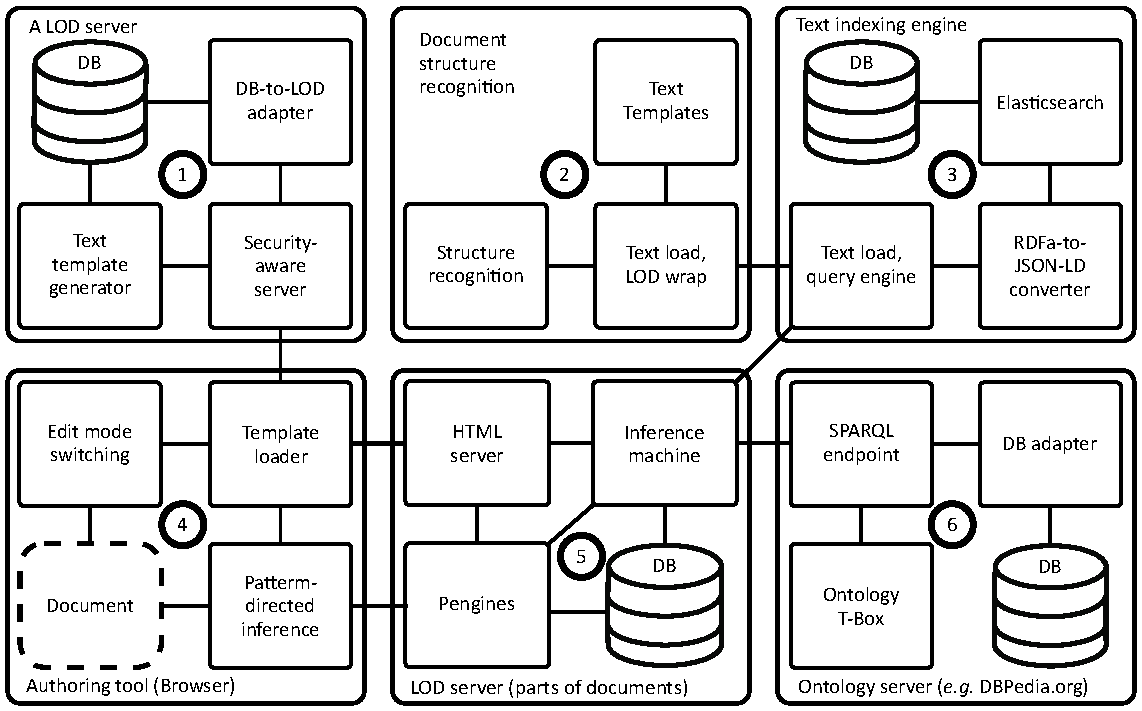
\includegraphics[width=1\linewidth]{architecture-mda-lod-ext.pdf}
  \caption{Architecture of digital archive tool set} \label{fig:arch}
\end{center}
\end{figure}

The toolkit consists of the following main components (fig.~\ref{fig:arch}):
\begin{itemize}
\item content and metadata repository with SPARQL and full--text search; the engines for LOD processing, based on the logical inference;
\item service for analysis of the stored content enriching the archive with semantic information describing the content;
\item tools for development of LOD applications and their user interfaces;
\item browser based authoring tools.
\end{itemize}

All components interact by means of network protocols and use utf-8 encoded HTML, TXT, XML and JSON formats for data representation, which are expressive enough and easily debugged.  Inference engines also support SPARQL protocol for issuing subqueries.

\subsection{Storing LOD documents}

The document content is stored either in the Kyotocabinet key-value database, either as a file in a file system.  Metainformation obtained by processing and analyzing a document is a content annotation and is described according to LOD standard vocabulary \textbf{oa} as a subgraph.

Each annotation (subject) is a tree with at least two nodes formed by the relations \texttt{oa:hasTarget} referring the original content and the \texttt{oa:hasBody} referring the annotation.  The text content of the document, if it has been acquired, is the document annotation as well as a structure of type Dublin Core (\textbf{dc}) describing metainformation found.  The contents (bytes, text) stored in Kyotocabinet is identified by its 128-bit Murmur3 hash function that allows us to create a reference key (hash) to the contents and in the backward direction.  Using such hashing allows us to simply and effectively implement computational mapping at a sufficiently low probability of clash of hash values.

Let us list the basic properties of used vocabularies in description of the content.

Open Annotation (\textbf{oa}). The vocabulary standard is adopted in 2017 by OMG, it is used to represent the content annotation describing other content.  A browser bookmark is an example of such content.

Friend--of--a--friend (\textbf{foaf}) allows one to describe information about agents: physical and legal entities, software agents.

Provenance (\textbf{prov}).  The \textbf{prov} ontology is the base of a description of information flows in documents and their relationships. The \textbf{prov} vocabulary is used to associate the document and owner organization or physical entity.

Dublin Core (\textbf{dc}) represents metainformation about the creative work: authors, format, contents, description, \emph{etc}.

DBpedia resource (\textbf{dbr}) is the namespace of the objects (resources) of Wikipedia.  The \textbf{dbr} ontology is used to refer to a specific entity, geographical names, \emph{etc}.

Schema.org (\textbf{schema}) represents the objects that are recognized by the crawlers of Google, Yandex, Yahoo, \emph{etc}.

In addition to these ontologies, we use standard ontologies (RDF, RDFs, RDFa, XSD) and ontologies from the NEPOMUK project (\url{https://userbase.kde.org/Nepomuk}), describing objects stored in the full-text indexes of digital archives.

\subsection{Component of content analysis}

Metainformation about the content is enriched with results of the analysis by so-called extractors. The extractors analyze the content and try to acquire information about text content, author, time of content creation, format, \emph{etc}. Extractors are implemented with the Linux utilities such as \texttt{file}, \texttt{extract} (\texttt{libextract}), \texttt{tracker} and \texttt{recoll}.  All these utilities are free software and integrated with the component as external processes.

The results of the extractor analysis are presented as a subgraph \textbf{oa}, associated with the source content and stored in a metadata repository of LOD.

\subsection{The metadata storage}

The implementation of metadata LOD graph storage is realized using ClioPatria \cite{b8} ontology server.  The ClioPatria system is implemented in the SWI--Prolog programming environment.  The project is under active development and aims to create a LOD graph storage service, implementing all the standards of storage and access, together with tight Prolog interpreter integration.

The system storage tier is implemented in C programming language.  The store uses compact data structures to represent triples in RAM and on hard disk.  A special feature of the storage is the fact that all triples are stored directly in RAM, as the service has no special assumptions about the structure of queries, which can be issued by client software.  Thus, server memory space is a critical resource of the repository.

ClioPatria developers implemented repository accessing in several ways: the SPARQL queries according to a standard protocol, direct queries to the ClioPatria Prolog subsystem using Pengines Protocol \cite{b9}.  For the Pengines protocols a number of APIs has been created for object--oriented programming languages such as JavsScript, Java, Python.  Using API classes, application developers and software agents are able to interact with the logic inference engine of the ClioPatria server.

\subsection{The inference machine}

Availability of ClioPatria's embedded programming system of SWI-Prolog \cite{b10} and the integration with RDFa allow one to process the marked up digital information stored in the archive on the base of logical inference.  Prolog allows us to make queries in SPARQL and Datalog formats, as well as to build a knowledge system to process the received data.

As an experiment, in a very short time, we managed to integrate well known Turbo Prolog 2.0 example of a natural language interface to a database on the US geography with ClioPatria's built in SWI-Prolog RDF system.  As a result, we developed a prototype with similar interface to a database of active faults of Siberia, aggregated at the Institute of the Earth crust SB RAS.

The server inference machine is used as regular engine of information processing at server side, resulting in set of variables of a query, which are filled in at the client side (browser) or templates at the server.  The graph of document data at server forms fact set of the Pengine's Prolog interpreter.  The set of rules are stored at server or sent with a query from browser.  Pengines allows us to store Prolog rules and queries in \texttt{<stript>} tag text.

\subsection{Full-text search}

The ClioPatria system has instruments of searching the text information for keywords, however, we added a more powerful system of Elasticsearch full-text index engine \cite{b13}.  Integration of this service is quite simple, since every RDF graph is representable as a JSON--LD object, while JSON is the primary format for storing indexed information in the ElasticSearch search engine; it is only necessary to separate a particular triples on the server responsible for the representation of the resource to the user in the search results.  Elasticsearch has the means of fuzzy comparison of terms that allows developing search subsystems retrieving relevant information.


\subsection{Tabular data interpretation}

Stored documents may contain a lot of useful information in their tables.  Extraction and understanding tabular data allows one to improve their semantic interpretation and get more qualitative metadata.  To extract information from tables we should detect them, recognize their structure, implement a structural analysis, and provide logically related data for further processing \cite{Shigarov_2017}.

Table structure recognition task consists in detection and extraction different structural elements such as cells, entries, labels, and categories.  Detection of structural and semantic elements of a table is carried out with a set of rules in the CLR language.  The rule engine is realized as a network service, it matches available facts of table elements against rules.  As a result, we get new facts about matched structure elements.  Recognition of semantic elements allows us to present table in a canonical form, with topmost row containing attribute names, and the remaining rows being a data record.  The attribute row refer cell columns and is associated with a categories, which are hierarchically organized, containing semantic labels.  Thus, data records present recovered relationships between their attribute labels in  categories.  Usually each data record is unique within a canonical table \cite{Shigarov_2016}, resulting in a possibility for restoring semantic relationships between elements of a table and their further mark--up and interpretation.  The corresponding conversion procedures are also implemented, producing various forms of rational tables.

\section{Application}

The designed tools used in solving a number of applied tasks built out of digital archive services, LOD and content processing components.

The Ministry of education and science of the Russian Federation incorporate the Bologna process in the educational environment of the Russian Federation.  One of the tasks solved is the transition to competence--oriented representation of the requirements to the pedagogical process.  The reform affects all aspects of the process, including the system of classification of specialties.  Various new classifications are introduced in curriculum, including programs and directions of a course set, specialization according to skill levels (bachelor, master degrees, \textit{etc}.  Applied bachelor degree has been added, as well as list of courses, aims and objectives of the courses (negotiation with the competencies specified in the Federal standard), forms of conducting classes in universities (introduction of interactive forms of learning), the distribution of lectures and practical sessions.  The existing documentation is supplemented by new forms of mandatory documents: the Fund of Assessment Means (FAM) and annotations of the courses.  In addition, the university management with the aim of improving the quality of educational services introduced its own improvements to form, content and document design requirements, in particular, to the quality of the conversion to HTML for publication on the website of an university.

For the minimum requirements fulfillment of the university management for each course, the instructor is required to prepare at least three documents: working program of the course, summary annotation, and  FAM.  This set is realized for each possible parameters combination of a course: the university, department, specialty, direction (profile), program, qualification (bachelor, specialist, undergraduate, graduate), academic or applied version of the qualification, form of study (full-time, part-time, evening, \emph{etc}.).  Each combination is reflected in the curriculum of the university, whose data is annually or twice a year being actualized in the work programs.

The last five years showed the level of maturity of decisions made by the managers of the Ministry in terms of requirements to the presentation of the course -- four generations of the standards (1, 2, 3 and 3+) were developed.  Each update required resubmission of the documents in the appropriate new form.  The task of developing new handbook now seems more simple than before as compared to the fulfillment the course documentation requirements.  Experience shows that most instructors are not able to cope with high-quality paperwork in the given time constraints, thus requiring the departments to hire a secretary, whose function is to bring documentation to the required quality level.

The solution to this problem consists in developing a software system that allows instructors to collect the texts of the work programs, abstracts and FAMs from separate parts: a list of competencies and curriculum; contents (subjects of taught module/course) and FAM, which are shared between different versions of documents.  The title pages are generated also from data of curriculum and templates set by the management.  Microsoft Word and Excel tools, that are commonly used for this task including built in VBA, are clearly not enough to support problem solution.

Consider the scheme of construction of marked up work program as an HTML page with the proposed system.  The presentation format is based on the results presented in \cite{b4,b15}.

%\begingroup\normalsize
% \begin{verbatim}
\begin{minted}{xml}
<!DOCTYPE html PUBLIC "-//W3C//DTD XHTML 1.0 ...>
<html lang="ru" xmlns=http://www.w3.org/1999/xhtml
xmlns:taa=http://irnok.net/engine/rdfa-manipulation
xml:lang="ru" metal:define-macro="page">
<head>
<!-- Connecting stylesheets and modules -->
</head>
<body prefix="rdf: http://www.w3.org/1999/...-ns#
foaf: http://xmlns.com/foaf/0.1/ imei: imei.html#
course: https://irnok.net/college/plan/01..16-...\
%D0\%BA_PB-SM.plm.xml.xlsx-....2.3.1.html#"
resource="#post"
typeof="schema:CreativeWork sioc:Post prov:Entity">
<!-- The application control panel -->
<main lang="ru" resource="#annotation"
typeof="oa:Annotation" id="main-doc-container">
<div property="oa:hasTarget" resource="#course-
work-prog"></div> <article property="oa:hasBody"
typeof="foaf:Document curr:WorkingProgram"
resource="#course-work-program" id="main-document">
<div taa:content="imei:title-page"></div>
<div taa:content="imei:neg-UMK"></div>
<section id="TOC" class="break-after">
<h2 class="nocount c">Table of Contents</h2>
<div id="tableOfContents"></div>
</section>
<section id="course-description"
  resource="#description"
  property="schema:hasPart"
  typeof="schema:CreativeWork">
<div property="schema:hasPart" resource="#purpose"
  typeof="dc:Text cnt:ContentAsText" >
<div property="cnt:chars"
  datatype="xsd:string">
<h2 property="dc:title"
  datatype="xsd:string">Aims and objectives of the
discipline (module)</h2>
<p>The aim of teaching the discipline ...</p>
</div> </div>
. . . . . . . .
\end{minted}
%\endgroup

In the example, the key structures are started from \texttt{taa:} prefix. Let us comment the structures.

The page displayed to the user is the abstract of the document ``\texttt{\#annotation}'', and both the annotated content and the annotation text is the same at the stage of authoring the document -- resource ``\texttt{\#course-work-program}''.  In LOD, all resources are global.  This is achieved by substitution of the default namespace (the URI of the current page) at the left side of the name of the resource.

The title page and the approval sheet are inserted from the templates page ``imei.html'' (information about the Institute of mathematics, economics and informatics of Irkutsk state university\footnote{\url{http://math.isu.ru}}).  The course data and the name of the specialty is filled in the templates from the context of the main document.  All the key static templates of courses can be placed in one page of templates.  The parts of the templates are arranged with a browser pattern-directed event-driven inference machine, implemented with JavaScript and special libraries, implementing HTML page loading.

The text is divided into sections, surrounded by tags \texttt{<div>} and \texttt{<span>} with the relevant RDFa structures.  Analysis of the experience of the developers LOD resources has shown that for the formation of the relationship is sufficient to use RDFa attributes \texttt{resource}, \texttt{property}, \texttt{typeof} and \texttt{datatype}.  The use of \texttt{rel} and \texttt{about} attributes are recommended to be abandoned.  This makes the structure of semantic markup more clean by reducing the number of used entities.

Attribute \texttt{taa:content} adds to the document a text from another HTML page, whose address is formed by the interpretation of the attribute, for example, \texttt{taa:content="course:time-distrib"} loads the text of a page generated by the table of distribution of time spent between the types of classes (lectures, practice, laboratory, independent work, \emph{etc}.).  To generate such tables, a web server has been realized for serving web pages of these courses. Each page represents a course/module, scheduled in the curriculum.  The page content is encoded by the structure of its URL and rendered at the time of first request.  Text templates are identified by the \texttt{id} attribute.

The presented approach supports various language processing for Russian, for example, declination of nouns, pronouns, participles and other words.  For this purpose, a \texttt{data-<command>} attribute HTML extension, JavaScript browser support, and a language service are implemented, where the linguistic processing queries are sent from browser to  service.  The attribute combinations define structural language morphological relations, which are interpreted by JavaScript routines.

In the text content edit mode, the work program tags combination with attributes \texttt{property="cnt:chars"} and \texttt{datatype="xsd:string"} denote conversion of their texts to editable form.  For clarity, the document without \texttt{taa:} inclusions is shown to the user, indicating these inclusions with the special tags and styles.  At the end of editing, the text is stored in the server file system.  The user can then commit the changes and sync the text of the saved document to the server control versions (git).

\subsection{LOD markup output}
\label{sec:lod-out}

Resulting HTML document is exported in Word and Excel formats.  LOD markup is dome with comments of a special ``\_\_RDF\_\_'' user and contains list of \texttt{<RDFa attrinute>=<value>} pairs or Turtle sentences.  Some RDFa key-value pairs refer the commented Word document text as a relation literal value.  RDFa attribute name is written in form of RDFa of Turtle resource notation.

The comments are hierarchically interpreted, giving rise the relation structures of the markup.  Printing documents is done with comments switched off, so a regular user is not disturbed with uncommon view full of comments.

Excel table exports can be marked up also with ``Defined ranges'' names.  Names of the ranges and the ranges are obtained from original LOD markups.  In this case the data exported can be directly used as input data for other table computations.

\subsection{Accounting data collection}
\label{sec:accounting}

Another example of the technology application is a software for accounting data collection.  In Russia there are a number of small-to-middle sized enterprises accounting software vendors, with market prevailing 1C.  The 1C software automating wide aspects of enterprises activity including accounting, logistics, human resources departments, school curriculum, \textit{etc}.  However, the cost of the software even for schools is high, and Irkutsk City council decided to reduce expenses with removing 1C accounting software and organize five Centralized accounting organizations.

In order to provide the service accountants must collect data from inferior organizations (schools, kindergartens, \textit{etc}.).  Data must be collected monthly, as well as upon a request from superior organizations (committees).  By means of our LOD software we developed web-services, which automate this process.

At the first stage, account creates Excel page, which will represent results of data collection in form of a report document.  The page can contain formulae calculating derivative values and aggregates, \textit{e.g.}, totals, which must be expressed using ``Defined ranges''.  Each define located withing the special define, named \texttt{REPEAT} is the data value to be collected.  The \texttt{REPEAT} defines parts of the Excel page, which is repeated for each organization's collected data.

The second stage is data collection itself, where the page is converted into a HTML form, which is shown to inferiors to fill in.  At the last stage, the collected data is used to construct the Excel page repeating sections.  The defines within \texttt{REPEAT} are corrected to contain all values for each organization, so aggregate formulae are not changed.

The data now can be imported to accounting software either from a rational table of collected values or from Excel report.  In the last case a special dictionary is used to relate defines with LOD relations.  The LOD published collected data is data sources for other documents.

The project sources are accessible via \url{https://github.com/isu-enterprise}.

\section{Conclusion and further development}
\label{sec:conc}

The paper discussed the facilities of the use of Linked Open Data (LOD) technologies for the solution of tasks of organizing digital document archives with instrumental tools for creating new documents based on the stored data.  Layout is carried out using algorithms that interpret the relationships between the elements of the HTML tree.  The layout algorithms are triggered in the presence of corresponding conditions in the nodes of the document tree. Each algorithm makes changes in the tree, resulting the final content and styles of the document. Forming documents are stored on servers that support the HTTP Protocol.  Tho applications are presented.

% An example of use of the development tools for the document synthesis in the educational environment and legal documents has been presented.
Further development of this project is carried in the following directions: a) improvement of the tools of typesetting documents, b) automation of the layout based on analysis of changes in the documents \cite{b2}, c) collecting of additional information about user needs, d) develop a regulated access to information stored in digital archives.  The created software tools and technologies aimed at the development of a software infrastructure of a global electronic document flow, allowing individuals and organizations to share documents, whose logical structure is partially formalizable within the framework of the traditional software of document automation.

\section{Acknowledgments}
The contribution of this work was supported by the Russian Science Foundation, Grant No. 18--71--10001.

% The results are obtained with the active use of the network infrastructure of Telecommunications of Center of collective use ``Integrated information"=computing network of Irkutsk scientific"=educational complex'' (\url{http://net.icc.ru}).

\begin{thebibliography}{99}
\bibitem{b1} Bizer Ch., Heath T., Berners-Lee T. Linked Data -- The Story So
  Far // International Journal on Semantic Web and Information Systems.
  2009. Vol. 5 (3). P. 1--22. \doi{10.4018/jswis.2009081901}.

\bibitem{c6} N.Heino, S.Tramp, N.Heino, S.Auer. Managing Web Content using Linked Data Principles – Combining semantic structure with dynamic content syndication. Computer Software and Applications Conference (COMPSAC), 2011 IEEE 35th Annual. pp. 245 - 250.  \url{http://svn.aksw.org/papers/2011/COMPSAC_lod2.eu/public.pdf}  Last accessed 30 May 2013.
\bibitem{b6}
  Baiju M. A Comprehensive Guide to Zope Component Architecture.
\url{http://muthukadan.net/docs/zca.html}. Last accessed 01 July 2017
\bibitem{b14}
  Capadisli, S., Guy, A., Verborgh, R., Lange, C., Auer, S., Berners-Lee, T.: Decentralised Authoring, Annotations and Notifications for a Read-Write Web with dokieli, Procs of ICWE international conference, 5-8 June, 2017, Rome, Italy. p. 469--481 URL: \doi{10.1007/978-3-319-60131-1_33}
\bibitem{b2}
  Cherkashin, E. A., Belykh, P. V. et al. An approach to managing a site
  content on the base of RDF technologies // Materials of All-Russian
  conference with international participation "Knowledge -- Ontology --
  Theory" (KONT-2013), 8 -- 10 October. Vol. 2. Novosibirsk.
  Publishing house "AIC Price-courier" (2013)
\bibitem{b3}
  Lehmann J., Isele R., Jakob M., Jentzsch A., Kontokostas D., et al.
  DBpedia -- A Large-scale, Multilingual Knowledge Base Extracted from
  Wikipedia // Semantic Web Journal. Vol. 6, No. 2, P. 167--195,
  IOS Press (2015)
\bibitem{b4}
  Krötzsch M. How to use Wikidata: Things to make and do with 40 million
  statements // In Keynote at the 10th Wikimania Conference. (2014).
\bibitem{b5}
  Daiber J., Jakob M., Mendes P. Improving Efficiency and Accuracy in
  Multilingual Entity Extraction // Proceedings of the 9th International
  Conference on Semantic Systems (I-Semantics) (2013)
\bibitem{b7}
  Langtangen H. A Primer on Scientific Programming with Python (Texts in
  Computational Science and Engineering) 3rd ed. Springer. 798 P. (2012)
\bibitem{b8}
  Wielemaker J., Beek W., Hildebrand M., Ossenbruggen J. ClioPatria: A
  SWI-Prolog infrastructure for the Semantic Web // Semantic Web.
  Vol. 7(5). P. 529--541 (2016) \doi{10.3233/SW-150191}
\bibitem{b9}
  Lager T., Wielemaker J. Pengines: Web Logic Programming Made Easy //
  Theory and Practice of Logic Programming. Vol. 14(4-5) (2014)
DOI: \doi{10.1017/S1471068414000192}
\bibitem{b10}
  Wielemaker J., Schreiber G., Wielinga B. Prolog-Based Infrastructure
  for RDF: Scalability and Performance // In: Fensel D., Sycara K.,
  Mylopoulos J. (eds) The Semantic Web -- ISWC 2003. ISWC 2003. Lecture
  Notes in Computer Science. Vol. 2870. Springer, Berlin,
  Heidelberg, 2003.
% \bibitem{b11}
%   Nefedova,Yu. S. The architecture of hybrid Recommender system GEFEST
%   (Generation--Expansion--Filtering--Sorting--Truncation) // Systems and
%   software of Informatics. 2012, vol. 22, issue.2, pp. 176--196.
% \bibitem{b12}
%   Beel J., Gripp B., Langer S., Breitinger C. Research-paper recommender
%   systems: a literature survey // International Journal on Digital
%   Libraries. 2016. Vol. 17. P. 305. doi:10.1007/s00799-015-0156-0.
%   (access date - 12.12.2016)
\bibitem{b13}
  Kuć R., Rogoziński M. Mastering Elasticsearch - Second Edition. Packt
  Publishing. 372 p. (2015)
\bibitem{Shigarov_2017}
Shigarov, A. O., Mikhailov, A. A. Rule-based spreadsheet data transformation from arbitrary to relational tables. Information Systems, 71, (2017). \doi{10.1016/j.is.2017.08.004}
\bibitem{Shigarov_2016}
Shigarov A.O., Paramonov V.V., Belykh P.V., Bondarev A.I. Rule-Based Canonicalization of Arbitrary Tables in Spreadsheets. In: Dregvaite G., Damasevicius R. (eds) Information and Software Technologies. ICIST 2016. E. Cherkashin et al.Communications in Computer and Information Science, vol 639. Springer (2016) \doi{10.1007/978-3-319-46254-7}
\bibitem{b15}
  Heino N, Tramp S, Auer S, et al. Managing Web Content using Linked
  Data Principles -- Combining semantic structure with dynamic content
  syndication // Computer Software and Applications Conference
  (COMPSAC), IEEE 35th Annual. 2011. P. 245-250.
  \url{http://svn.aksw.org/papers/2011/COMPSAC\_lod2.eu/public.pdf}. Last accessed 30 May 2013.
\end{thebibliography}
\end{document}

%%% Local Variables:
%%% mode: latex
%%% TeX-master: t
%%% End:
